\documentclass[letterpaper, 11pt]{article}

% set version variable
\newcommand{\versionnumber}{0.1}

% russian language
\usepackage[utf8]{inputenc}
\usepackage[T2A]{fontenc}
\usepackage[english, russian]{babel}

% math
\usepackage{mathtools}
\usepackage{amsmath}

\usepackage{amssymb} % some math symbols
% abs function
\DeclarePairedDelimiter{\abs}{\lvert}{\rvert}

% enumerate
\usepackage{enumerate}

% set type and margins of the page
\usepackage{geometry}  % document margins
\geometry{letterpaper, left=1.4in, right = 1.4in, top = 1.7in, bottom = 1.7in}

% color links in content
\usepackage{hyperref}
\hypersetup{
    colorlinks=true,
    linkcolor=red,
    urlcolor=blue,
    linktoc=all
}

% indent at first \par after section
\usepackage{indentfirst}

% fixed table and figures in section
\usepackage{float}

% colors
\usepackage{color}
\usepackage[usenames,dvipsnames]{xcolor}

% paragraph indent
\setlength{\parskip}{0.5em}

\title{\large{Краткий конспект}\\
\LARGE{Лекция 1. Поиск мотивов}\\
\normalsize версия \versionnumber (\textcolor{NavyBlue}{незавершенная})}
\date{11 февраля, 2016}
\author{Д. Ищенко\thanks{МФТИ} \and Б. Коварский\footnotemark[1]
\and И. Алтухов\footnotemark[1] \and Д. Алексеев\footnotemark[1]}

\begin{document}
\maketitle
\thispagestyle{empty}
\clearpage

% let's go
\section{Зачем искать мотивы?}
\section{Несколько слов о сложности алгоритмов}
\par
При разработке алгоритма важно представлять и оценивать кол-во времени 
необходимое для его исполнения при конкретных входных данных, а также объем компьютерных ресурсов,
задействованных при исполнении алгоритма. Когда мы говорим про <<конкретные данные>>, мы подразумеваем, 
определенную величину, например, размер памяти выделяемой под входные данные в битах. Будем называть эту
величину $n$. Для простоты будем считать, что время необходимое для исполнения алгоритма \textit{пропорционально}
кол-ву элементарных операций (которые в свою очередь определены архитектурой процессора). Будем считать
элементарными операциями: сложение, вычитание, умножение, деление, вычисление корня. Тогда оценка 
времени сводится к определению $f(n)$, функции количества элементарных операций от размера входных данных. Нас не будет 
интересовать точное значение $f(n)$ (это и не всегда возможно определить), а только лишь его оценка (чаще всего оценка сверху). Определяется она с помощью термина <<$O$ большое>> для ассимптотического поведения функций.
$f(n) = O(g(n))$ означает, что кол-во операций $f(n)$ при увеличении $n$ будет возрастать не быстрее, чем $g(n)$ умноженная на некоторую константу.
\[
\exists (C > 0), n_0 : \forall (n > n_0) \; f(n) \leq Cg(n)
\]
\par
Напрмер, сложность алгоритма который вычисляет простую сумму $k$ входных чисел $a_k$ оценивается, как $O(k)$. Грубо говоря, мы выполняем $(k-1)$ операций сложения. Таким образом кол-во операций $f(n)$ будет возрастать пропорционально кол-ву входных чисел $k$. Объем входных данных в битах можем оценить, как некоторую константу (например кол-во бит, зарезервированных под одно входящее число) умноженную на их кол-во $n = c \cdot k$, тогда $f(n) = f(c \cdot k) = k - 1 = O(k)$. Рассмотрим другой пример, алгоритм находящий ... \textcolor{red}{алгоритм $O(n^2)$} ...
\par
Аналогичные рассуждения в оценке применимы и к вычислению необходимой памяти (чаще оперативной) выделяемой
при исполнении алгоритма. Оценивается кол-во выделяемых бит $m(n)$ от размера входных данных и оценивается с помощью
$O(p(n))$. Возвращаясь к алгоритму вычисления суммы $k$ чисел $a_k$. Допустим, алгоритм построен следующим образом: (i) прочесть все $k$ чисел и записать в массив, (ii) просуммировать все $a_k$ и результат записать в $s$, (iii) выдать результат $s$. Задействованная оперативная память -- величина $m(n) = m(k \cdot c) = k \cdot c + c = c(k + 1) = O(k)$ (нам необходимо записать в массив все $k$ чисел, каждое из которых занимает $c$ бит, а также выделить память для перемнной $s$ размера $c$ бит). Если же изменить алгоритм следующим оразом: (i) объявляется переменная $s = 0$ для хранения суммы, (ii) по-очередно читается одно число из $a_k$ и добавляется к $s$, $s = s + a_k$, после чего $a_k$ удаляется из памяти (iii) выводится $s$. То в такой реализации нам необходимо хранить всего два значения $s$ и текующее $a_k$, а значит всего $2c$ бит. Другими словами, кол-во необходимой памяти \textit{не зависит} от размера входных данных (кол-ва входных чисел), такой вариант оцениватся, как $m(n) = 2c = O(1)$. При этом в обоих реализациях алгоритма оценка времени одинакова $f_1(n) = f_2(n) = O(k)$.
\par
Идеальным случаем ... \textcolor{red}{написать про $O(n)$} ...
\section{Простой подход к поиску мотива}
\par
Вернемся к задаче о поиске мотива. Есть строка (геном) $S$ и паттерн (мотив) $M$:
\begin{verbatim}
 S :  TATGCATGCATGA
 M :  ATGCTGA
\end{verbatim}
\par
Необходимо определить все позиции вхождения $M$ в $S$. Рассмотрим самый простой алгоритм, заключающийся в полном переборе всех позиций в $S$, подставления в них $M$ и проверки попарных совпадений символов (нуклеотидов).
\begin{verbatim}
 S :  TATGCATGCATGA
M1 :  ATGCATGA
      * 
M2     ATGCATGA
       +++++++*
M3      ATGCATGA
        *
M4       ATGCATGA
         *
M5        ATGCATGA
          *
M6         ATGCATGA
           ++++++++
\end{verbatim}
\par
Обозначаем символом <<*>> проверку на совпадение, которая вернула значения $FALSE$ (символы отличаются), а символом <<+>> проверку, вернувшую $TRUE$ (символы совпадают). Алгоритм можно описать следующим образом: двигаемся 
\section{Усовершенствование простого подхода}
\par
\begin{verbatim}
 S :  TATGCATGCATGA
M1 :  ATGCATGA
      * 
M2     ATGCATGA
       +++++++*
M3         ATGCATGA
           ++++++++
\end{verbatim}

\par
\begin{verbatim}
S  :  TATGCATGCATGA
M1 :  ATGCATGA
      * 
M2     ATGCATGA
       +++++++*
M3         ATGCATGA
              +++++
\end{verbatim}
\par
Вышеописанные подходы позволоили нам уменьшить количество сравнений. Но это был частный пример и рассуждали мы в <<свободной>> форме, а хочется это формализовать в виде алгоритма.
\section{Z-алгоритм}
\par
Обобщение вышеописанных наблюдений формализуется в виде $Z$-алгоритма. Перед непосредственным разбором алгоритма, рассмотрим понятие <<предобработки>> (<<предпроцессинга>>) строки. Этот термин обозначает проведение каких-либо операций со строкой еще до исполнения самого алгоритма поиска мотива. Причем, предобработку можно проводить как самой строки $S$ (мы коснемся этого позже при разборе суффиксных деревьев), так и строки содержащей мотив $M$. Последний вариант мы разберем сейчас и убедимся, как такой подход позволит нам решить задачу поиска мотива за линейное время $O(n + m)$, где $n$ -- длина строки (генома) $S$, $m$ -- длина мотива $M$.
\par
Введем несколько определений:
\begin{enumerate}[(i)]
\item
\textbf{$k$-й префикс} строки $S$: подстрока длины $k$, начинающаяся с первого символа $S[1..k]$.
\item
Для строки $S$ и позиции $i \geq 2$, $Z_i(S)$ -- длина максимальной подстроки $S$, начинающейся с позиции $i$ и совпадающией с префиксом $S$ той же длины.
\end{enumerate}
\par
Рассмотрим строку $S$ и укажем различные значения $Z_i(S)$:
\begin{verbatim}
 S  :  ATGCATGCATGA
        |  |   | |
        |  |   | Z11 = 0
        Z2 = 0 |
           |   |
           |   Z9 = 3 [ATG]
           Z5 = 7 [ATGCATG]
\end{verbatim}
\par
Для лучшего понимания величины $Z_i(S)$ введем понятие $Z$-ящика ($Z$-box), каждый <<ящик>> начинается в некоторой позиции $i \geq 2$, в которой $Z_i > 0$, длина ящика соответствует значению $Z_i$.
\begin{figure}[H]
  \center{
  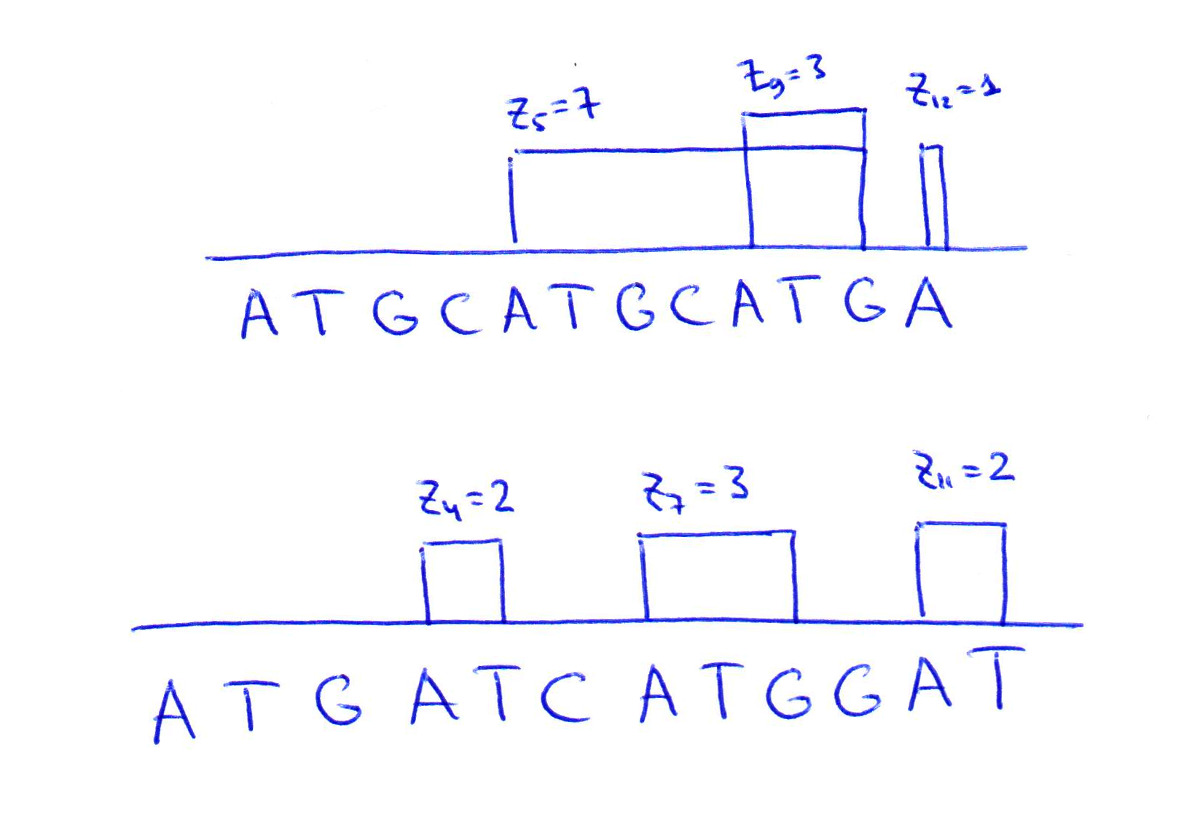
\includegraphics[]{fig/fig1.jpg}
  }
  \caption{Визуальное изображение значений $Z_i$ в виде $Z$-ящиков. Длина ящика соответствует значению $Z_i$, высота ящика смысла не имеет, и изменятеся \textit{только для удобства визуализации}.}
\end{figure}

\par
Введем еще две дополнительные величины, их осмысление потребует некоторой \textit{внимательности и усердия}:
\begin{enumerate}[(i)]
\setcounter{enumi}{2}
\item
Для любого $i \geq 2$, $r_i$ -- координата самого правого символа во всех $Z$-ящиках, которые начинаются в позициях $1 < j \leq i$
\item
$l_i$ -- это позиция, с которой начинается $Z$-ящик, которому соответствет $r_i$. В случае, если несколько $Z$-ящиков заканчиваются на $r_i$, выбирается наименьшая позиция.
\end{enumerate}
\par
Разберем несколько примеров определения $r_i$ и $l_i$ на рисунке:
\begin{figure}[H]
  \center{
  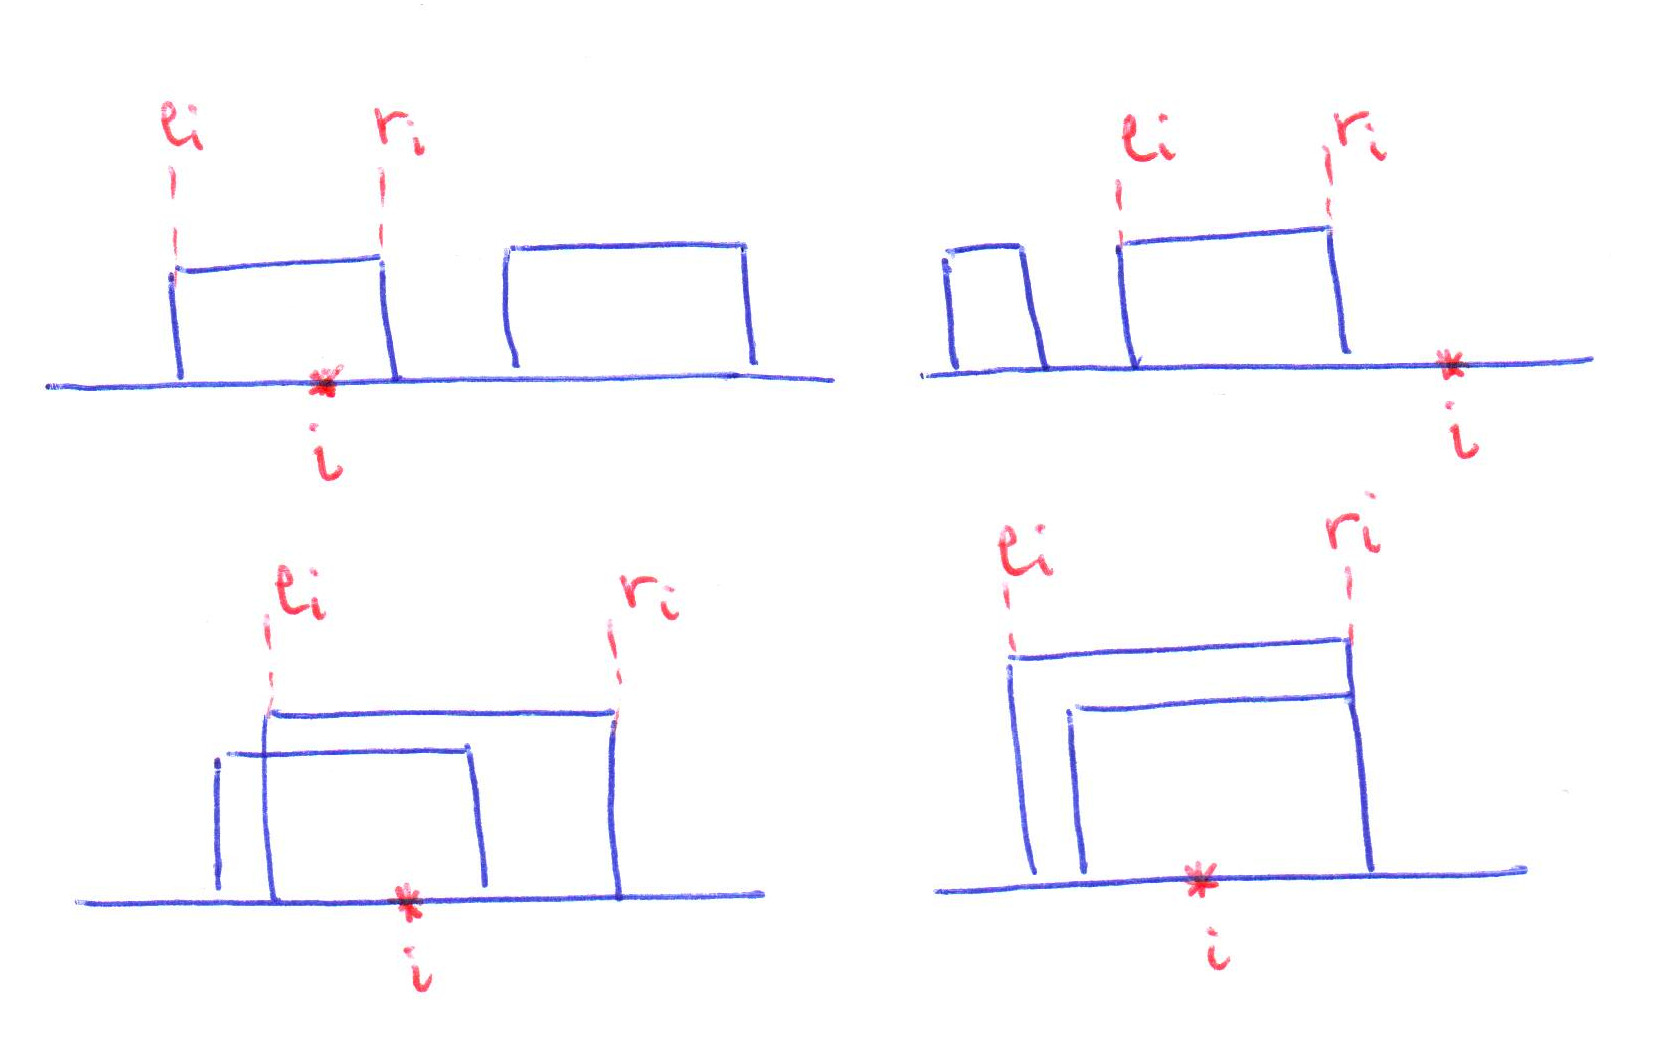
\includegraphics[]{fig/fig2.jpg}
  }
  \caption{Несколько примеров определения $r_i$ и $l_i$ для заданного $i$.}
\end{figure}
\par
Покажем, что вычисление всех значений $Z_i$ (что эквивалентно построению всех $Z$-ящиков) возможно за линейное время, т.е. $f(n) = O(n)$, где $n$ -- длина строки $S$. Сначала разберем частный случай, а затем перейдем к общему алгоритму.
\par
Для того, чтобы вычислить $Z_2$ достаточно сравнивать $S_k$ c $S_{k-1}$, начиная с $k = 2$, пока не дойдем до первого несовпадения. Автоматическим мы определяем и $r_2$ с $l_2$, $r_2 = z_2 + 1$, $l_2 = 2$. Если не совпадают даже $S_2 \neq S_1$, то $r_2 = l_2 = 0$.
\par
Теперь предположим, что мы находимся на $(k + 1)$-й позиции ($k = 100$), все значения $Z_2 .. Z_{100}$ уже известны и $r_k = r_{100} = 110, \; l_k = l_{100} = 80$ (значит есть <<ящик>> $Z_{80} = 110 - 80 + 1 = 31$) (Рис. 3). Стоит задача вычислить $Z_{101}$.
\begin{figure}[H]
  \center{
  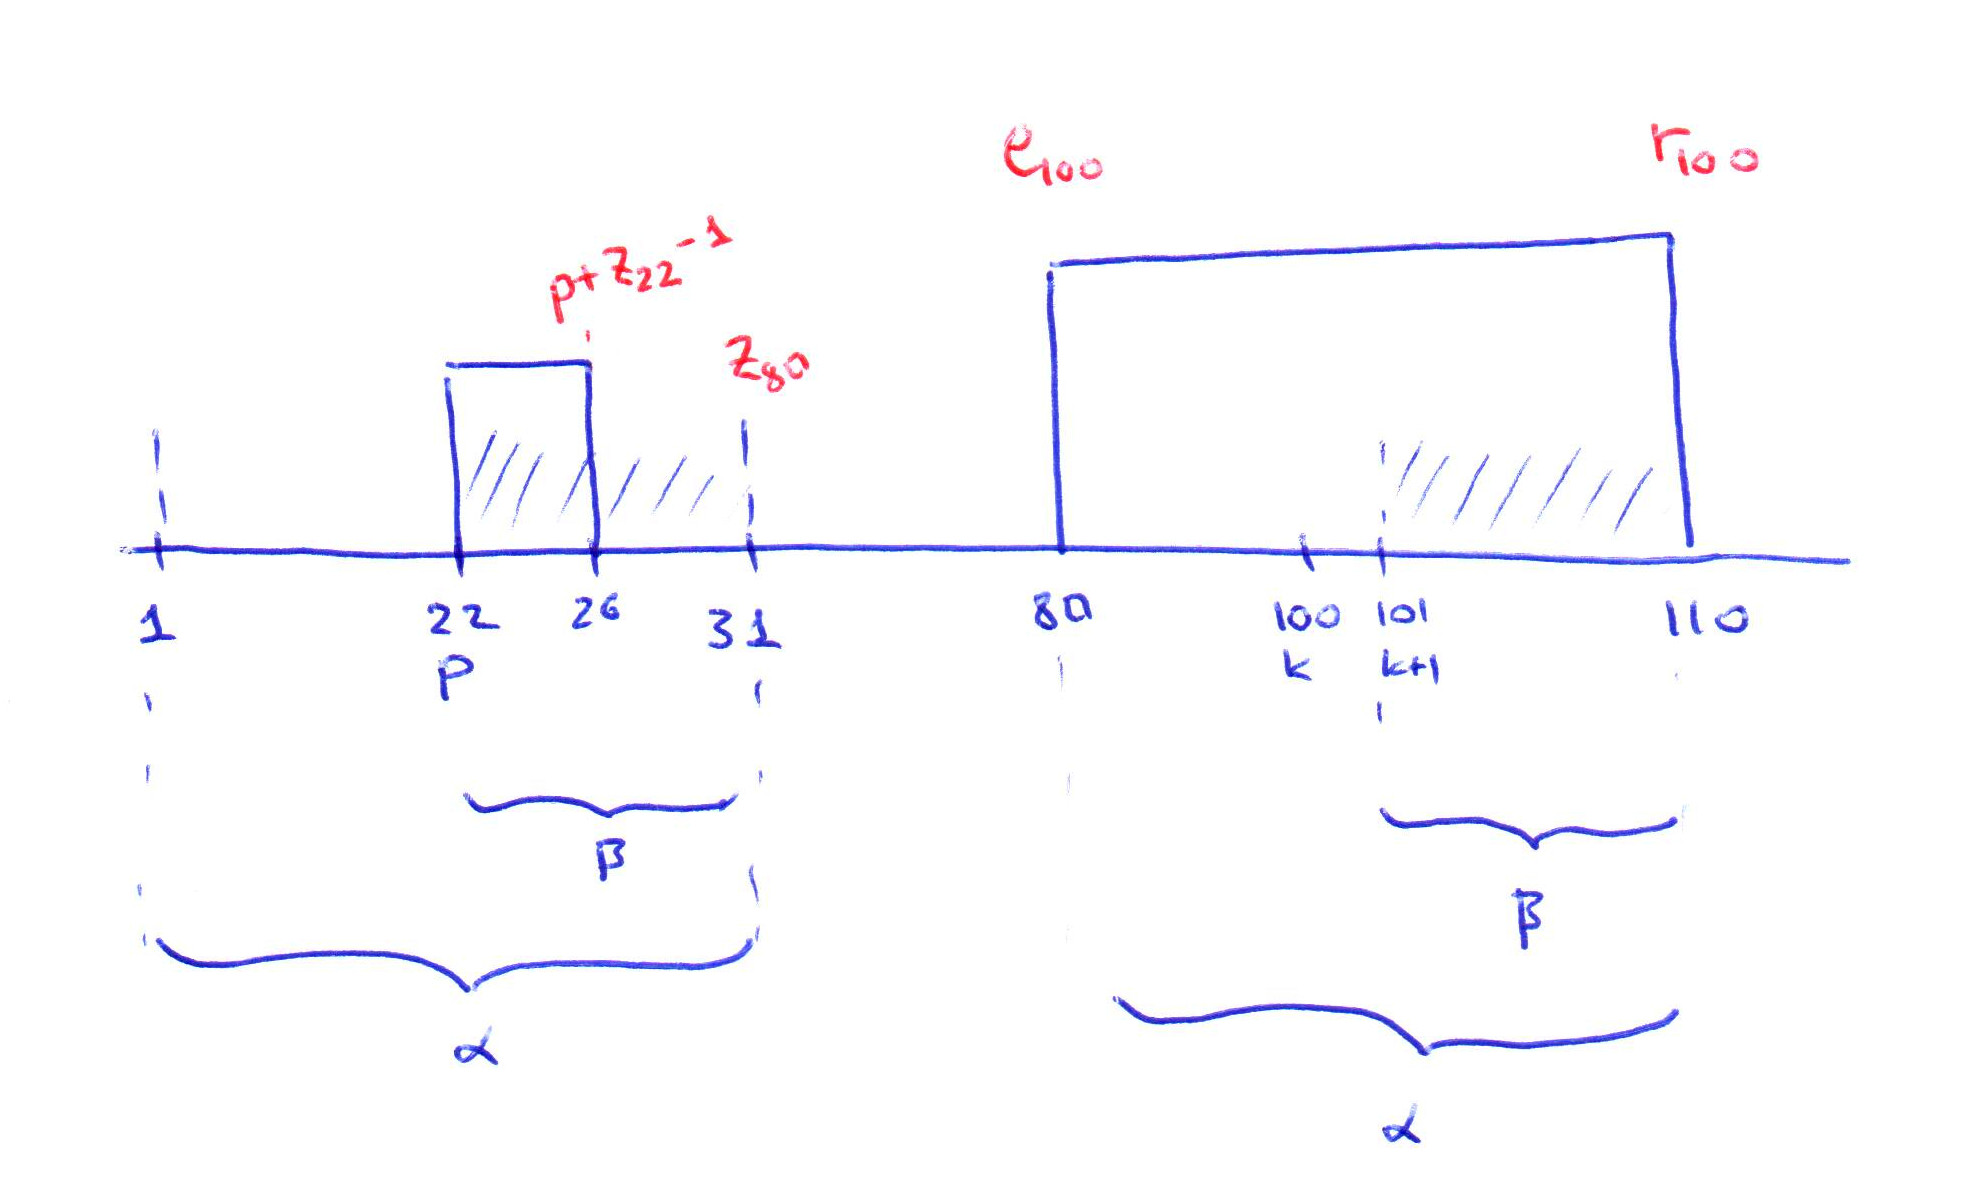
\includegraphics[scale=0.9]{fig/fig3.jpg}
  }
  \caption{Несколько примеров с указанными тройками $\{i, r_i, l_i\}$.}
\end{figure}
\par
Назовем последовательность $S[80..110] = \alpha$, тогда такая же последовательность $\alpha$ находися в начале строки $S[1..31]$ (по определению $Z$-ящика). Очевидно, что последовательность, начинающаяся с $k = 101$, $S[101..110]$, совпадает с $S[22..31]$ (соответствующие подпоследовательности $\alpha$), назовем их $\beta$. Для вычисления $Z_{101}$ достаточно посмотреть на значение $Z_{22}$ (ящика, начинающегося с 22 позиции). Пусть $Z_{22} = 5$, это значит, что начиная с символа $S_{22}$ только пять символов совпадают с префиксом ($S[1..5]$), т.е. мы автоматически вычисляем $Z_{101} = Z_{22} = 5$ без дополнительных сравнений символов (т.к. $Z$-ящик, начинающийся с 22-ой позиции, короче строки $\beta$, а строка начинающася со 101 позиции равна $\beta$.
\par
Мы рассмотрели важный частный случай, перейдем к формальному описанию алгоритма вычисления $Z_{k+1}$ элемента, при вычисленных $\{Z_1, Z_2, ..., Z_k\}$, $\{r_1, r_2, ..., r_k\}$, $\{l_1, l_2, ..., l_k\}$:
\begin{enumerate}[(i)]
\item
Если $k + 1 > r_k$ (ни один $Z$-ящик, не покрывает $(k+1)$-й символ), $Z_{k+1}$ вычисляется последовательным сравнением символов $S[k+1]$ с $S[1]$, $S[k+2]$ с $S[2]$ и т.д. до первого несовпадения. $Z_{k+1}$ будет равно кол-ву совпавших элементов, если $Z_{k+1} > 0$, то $r_{k+1} = k + Z_{k+1}$, $l_{k+1} = k + 1$.
\item
Если $k + 1 \leq r_k$ ($(k+1)$-й символ содержится в $Z$-ящике), подстрока $S[l_k..r_k]$ (назовем её $\alpha$) совпадает с префиксом $S$. Тогда $S_{k+1}$ совпадает с $p$-м символом, где $p = k + 1 - l_k + 1$. Строка $S[(k+1)..r_k]$ (назовем ее $\beta$) совпадает со строкой $S[p..Z_{l_k}]$. Это означает, что строка начинающаяся с позиции $(k+1)$ совпадает с префиксом хотя бы на $Z_{p}$ символов или длину строки $\beta$ (обозначим её $\abs{\beta}$). Рассмотрим два случая:
\begin{enumerate}
 \item
 $Z_{p} < \abs{\beta}$: тогда $Z_{k+1} = Z_{p}$, $r_{k+1} = r_{k}$, $l_{k+1} = l_k$.
 \item
 $Z_{p} \geq \abs{\beta}$: тогда $S[(k+1)..r_k]$ является префиксом $S$, и $Z_{k+1} \geq \abs{\beta} = r_k - k$. Но $Z_k$ может быть больше $\abs{\beta}$, поэтому начинаем сравнение $S[r_k + 1]$ с символвами $S[\abs{\beta} + 1]$, $S[r_k + 2]$ с символвами $S[\abs{\beta} + 2]$ и т.д. до первого несовпадения. Пусть несовпадение возникло в позции $q \geq r_k + 1$, тогда $Z_{k+1} = q - (k +1)$, $r_{k+1} = q$ и $l_{k+1} = k + 1$.
\end{enumerate}
\end{enumerate}
\par
Такой алгоритм найдет все значения $Z_k$ за линейное время $O(n)$, т.к. как каждый символ мы сравниваем только один раз с другим символом строки). А теперь вернемся к нашей задаче поиска мотива $M$ в последовательности $S$. Объединим строки $M$ и $S$ в одну, вставив между ними символ, который не встречается ни в $M$ ни в $S$ (если мы работает с нуклеотидными представлениями, то можно выбрать любой символ, отличный от A, T, G, C), например, <<\$>>:
\begin{verbatim}
M$S
\end{verbatim}
\par
А теперь применим алгоритм вычисления $Z$-значений для такой последовательности. Очевидно, что позиции вхождения $M$ в $S$ будут теми позициями, в которых $Z_k$ равно длине мотива, т.е. $Z_k = \abs{M}$. Вот и все.
\section{Ссылки}
\end{document}
